% Capitolo 4 generato dalla bozza Markdown verificata.
\chapter{Architettura proposta}\label{architettura-proposta}

\section{Architettura generale}\label{architettura-generale}

L'architettura proposta è organizzata in componenti con responsabilità distinte, progettati per elaborare le evidenze ricavate dalle catture di traffico e valutarle secondo i criteri definiti per ciascun test. Questa suddivisione permette di separare le regole specifiche dei singoli casi dalla logica generale del sistema, favorendo il riutilizzo dei componenti.

\begin{figure}[H]
\centering
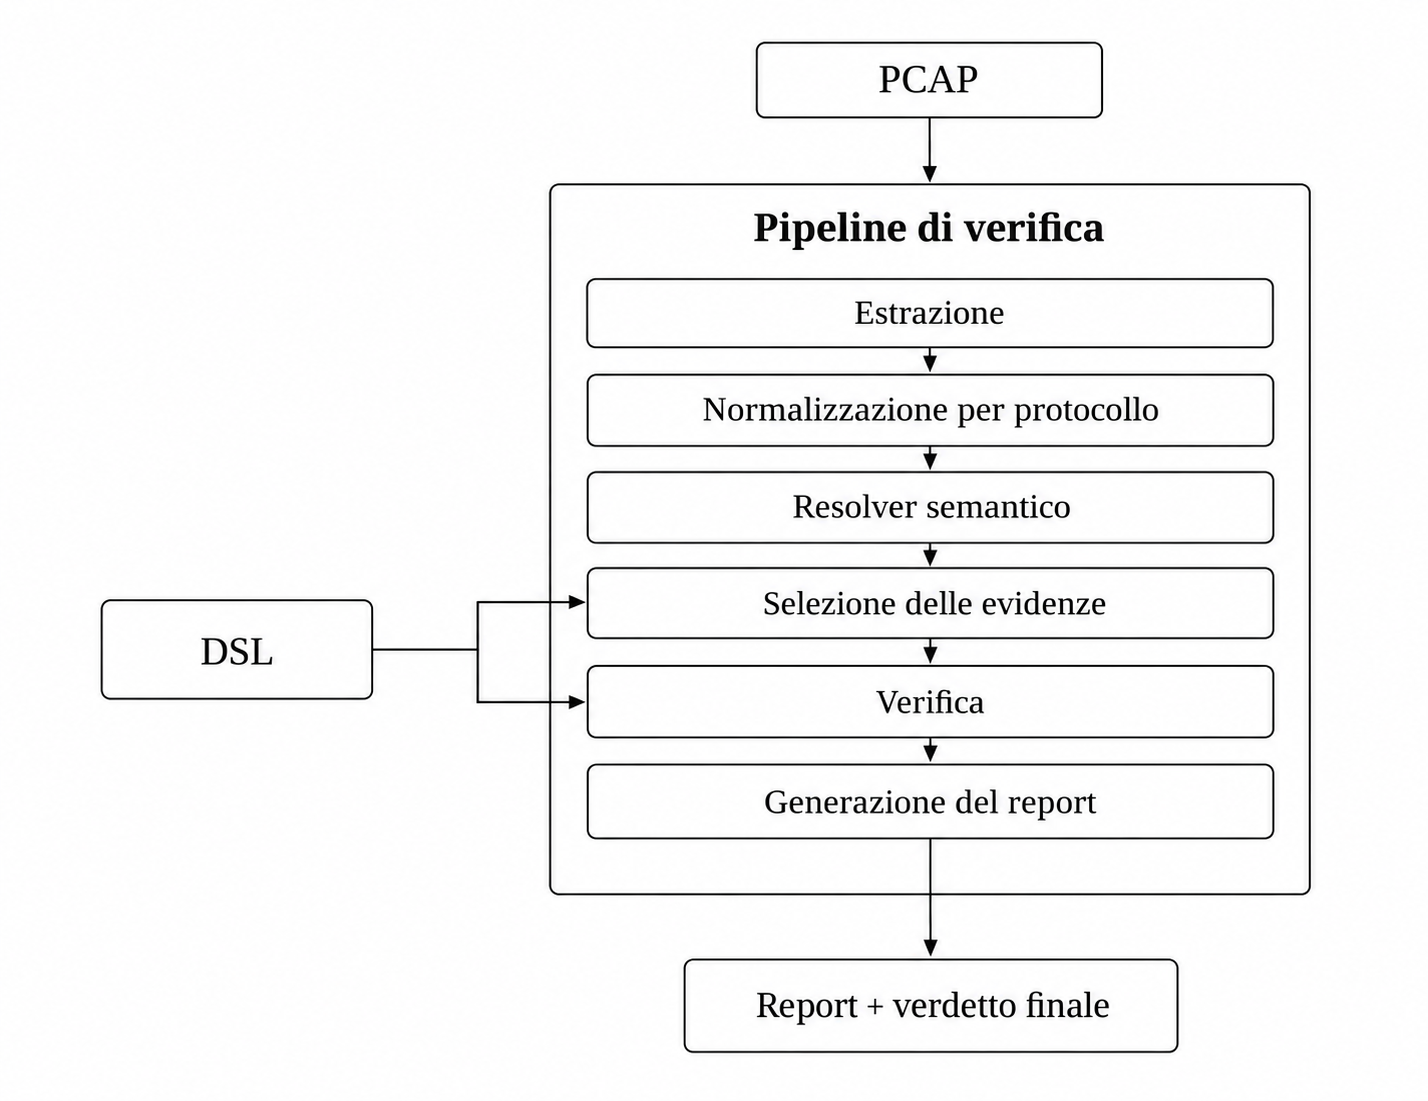
\includegraphics[width=0.94\textwidth,height=0.74\textheight,keepaspectratio]{figure/architettura_generale.png}
\caption{Architettura generale della pipeline di verifica degli esiti SCAS.}
\label{fig:architettura}
\end{figure}
\needspace{5\baselineskip}


Il sistema riceve due input principali: una cattura di traffico, contenente le evidenze da analizzare, e una specifica DSL, che definisce quali eventi individuare e quali condizioni verificare. Quest'ultima riveste un ruolo centrale nell'architettura, poiché guida la selezione delle evidenze e la successiva applicazione dei criteri, mentre la pipeline mette a disposizione i meccanismi comuni di elaborazione e verifica.

L'esecuzione è organizzata attraverso il file di configurazione \texttt{tests.json}, che associa a ciascun caso di test la cattura, la specifica DSL e i parametri necessari all'analisi. La Figura~\ref{fig:architettura} illustra l'organizzazione generale dell'architettura e le relazioni tra i suoi componenti.


\section{Estrazione strutturata del traffico}\label{estrazione-strutturata-del-traffico}

La cattura del traffico di rete effettuata durante un test viene conservata in un file PCAP, che costituisce la sorgente delle evidenze osservabili. Poiché le informazioni registrate non sono immediatamente disponibili in una forma adatta all'analisi, è necessaria una fase preliminare di estrazione che le renda accessibili in modo strutturato.

A tale scopo viene utilizzato TShark, un analizzatore di protocolli di rete che applica i \emph{dissector} dei protocolli presenti nella cattura e rende accessibili i relativi campi decodificati. L'estrazione avviene mediante l'opzione \texttt{-T\ ek}, che produce record strutturati in formato JSON, consentendo alla pipeline di operare sui campi decodificati anziché sui byte grezzi dei pacchetti. \cite{wireshark_tshark_docs}

I record prodotti contengono informazioni generali, come numero di frame, timestamp e indirizzi IP, insieme ai campi propri dei protocolli analizzati. La diversa organizzazione di questi campi rende necessaria una successiva fase di normalizzazione.

\section{Normalizzazione degli eventi}\label{normalizzazione-protocol-specifica}

La normalizzazione ha lo scopo di ricondurre le informazioni estratte dai diversi protocolli a una rappresentazione comune degli eventi di rete. Per ciascun protocollo supportato, un normalizzatore interpreta i campi disponibili e li organizza in un oggetto denominato \texttt{MessageEvent}, che raccoglie sia le informazioni generali dell'evento sia i dati specifici del messaggio.

La struttura del \texttt{MessageEvent} comprende i seguenti attributi:

\par\noindent\begin{minipage}{\linewidth}
\begin{lstlisting}
class MessageEvent:
    frame_number: int
    timestamp: float
    protocol: str
    kind: str
    
    src: str | None = None
    dst: str | None = None
    
    message_type: str | None = None
    
    related_frames: list[int] = field(default_factory=list)
    
    correlation: dict[str, Any] = field(default_factory=dict)
    
    fields: dict[str, Any] = field(default_factory=dict)
\end{lstlisting}
\end{minipage}\par

Nell'implementazione attuale sono previsti normalizzatori per NAS, HTTP/2 e PFCP.
\section{Risoluzione semantica}\label{risoluzione-semantica}

La normalizzazione produce eventi rappresentati secondo una struttura comune, ma in alcuni casi il loro significato applicativo non è ancora completamente esplicito. Ciò avviene soprattutto per messaggi relativi alle interazioni della Service-Based Architecture, dove i messaggi HTTP/2 possono rappresentare operazioni differenti in funzione del servizio richiesto e del contenuto applicativo.

Per gestire questa esigenza, viene introdotto un \emph{resolver semantico}, incaricato di interpretare gli eventi normalizzati e associarli a tipologie coerenti con il dominio 5G. Ad esempio, analizzando il percorso della richiesta HTTP/2, il resolver può riconoscere un'operazione di \emph{NF Discovery} presso l'NRF e classificare gli eventi correlati come \texttt{nrf.discovery.request} e \texttt{nrf.discovery.response}.

Il resolver opera quindi a un livello di astrazione superiore rispetto ai normalizzatori, in quanto non ricostruisce nuovamente i messaggi, ma utilizza le informazioni già disponibili per completarne l'interpretazione e rendere esplicito il tipo semantico degli eventi.

\section{Selezione dell'evidenza tramite DSL}\label{selezione-dellevidenza-tramite-dsl}

La normalizzazione e l'eventuale risoluzione semantica trasformano il traffico acquisito in una sequenza di eventi strutturati, tra i quali la fase di selezione individua quelli richiesti dal caso di test considerato.

Per descrivere le evidenze da individuare, il DSL mette a disposizione due costrutti principali: \texttt{SEQUENCE}, che permette di specificare una successione ordinata di eventi, e \texttt{COLLECT}, utilizzato per raccogliere più occorrenze di un determinato tipo di evento. Attraverso questi costrutti è possibile indicare quali eventi ricercare nella cattura e, quando necessario, le relazioni di ordine che devono sussistere tra essi.

Gli eventi individuati vengono associati a identificatori simbolici, denominati \emph{alias}, definiti nella specifica DSL. Un alias può rappresentare, ad esempio, un particolare messaggio riconosciuto tramite \texttt{SEQUENCE} oppure una collezione di messaggi ottenuta mediante \texttt{COLLECT}. L'associazione tra l'alias e l'evidenza corrispondente prende il nome di \emph{binding}.

I binding prodotti dalla selezione vengono raccolti nel \texttt{BindingContext}, una struttura che rende disponibili le evidenze individuate attraverso i rispettivi alias. I criteri di verifica possono così riferirsi direttamente agli eventi selezionati, indipendentemente dalla loro posizione nella cattura.


\section{Verifica}
\label{verifica}

Una volta costruito il \texttt{BindingContext}, la fase di verifica valuta l'evidenza selezionata rispetto ai criteri definiti nella DSL, al fine di stabilire se il comportamento osservato soddisfi le condizioni previste per il caso di test.

L'architettura prevede due modalità complementari: la verifica statica e la verifica temporale.

La prima opera sui valori associati ai binding, valutando proprietà e relazioni tra i dati estratti dagli eventi selezionati. È utilizzata, ad esempio, per controllare la corrispondenza tra valori o l'assenza di duplicati.

La seconda riguarda invece le relazioni temporali tra gli eventi, come il rispetto di determinati intervalli di tempo. Tali proprietà sono espresse mediante la \emph{Metric First-Order Temporal Logic} (MFOTL) e valutate attraverso il motore di verifica esterno MonPoly.

I risultati ottenuti dalle due modalità concorrono alla determinazione del verdetto complessivo del caso di test.


\section{Reporting}\label{reporting}

L'ultima fase dell'architettura riguarda la produzione del report, che affianca al verdetto le informazioni su cui esso si basa. Il reporter, comune ai diversi casi di test, organizza tali informazioni in un documento strutturato in formato \texttt{JSON}, distinguendo i dati relativi al test e all'esecuzione dai criteri valutati, dalle evidenze osservate e dal risultato complessivo.

\Needspace{16\baselineskip}
Il seguente schema illustrativo semplificato presenta i principali campi del report; i segnaposto indicano parti omesse e non costituiscono un documento JSON completo:

\par\noindent\begin{minipage}{\linewidth}
\begin{lstlisting}
{
    "metadata": {
        "generator": "generic_verification_pipeline",
        "tshark_version": "..."
    },
    "test": { "id": "..." },
    "source": { "pcap": "...", "sha256": "..." },
    "configuration": {
        "pipeline": "...", "rules": "...", "traffic": { }
    },
    "criteria": [ ... ],
    "verification": {
        "results": [ ... ],
        "overall_verdict": "PASS"
    },
    "evidence": { "bindings": { ... } },
    "explanation": { "summary": "..." },
    "verdict": "PASS"
}
\end{lstlisting}
\end{minipage}\par

Il report favorisce sia la verificabilità sia la riproducibilità dell'analisi. I criteri valutati e i riferimenti alle evidenze consentono di controllare le motivazioni del verdetto, mentre i metadati relativi alla cattura, alla configurazione e alla versione di TShark documentano alcune condizioni utili per ripetere la verifica. In particolare, l'hash SHA-256 del file PCAP permette di controllare che una successiva analisi utilizzi la stessa cattura.
